% % % % % % % % % % % % % % % % % % % % % 
% numerical.tex - Ian Huston
% $Id: numerical.tex,v 1.18 2009/10/05 18:19:11 ith Exp $
% % % % % % % % % % % % % % % % % % % % % 
% Redefine CVSRevision for this section
\renewcommand{\CVSrevision}{\version$Id: numerical.tex,v 1.18 2009/10/05 18:19:11 ith Exp $}
% \input{numerical/paper3}

% % % % % % % % % % % % % % % % % % % % % % % % % % % % % % % % 
% =========================================================== %
% % % % % % % % % % % % % % % % % % % % % % % % % % % % % % % %
\chapter{Numerical system and implementation}
\label{ch:numericalsystem}
% % % % % % % % % % % % % % % % % % % % % % % % % % % % % % % % 
% =========================================================== %
% % % % % % % % % % % % % % % % % % % % % % % % % % % % % % % %

\addtodo{Add intro to numerics}
% 
% 
% % % % % % % % % % % % % % % % % % % % % % % % % % % % % % % % 
% =========================================================== %
% % % % % % % % % % % % % % % % % % % % % % % % % % % % % % % %
\section{Introduction}
\label{sec:intro-num}
% % % % % % % % % % % % % % % % % % % % % % % % % % % % % % % % 
% =========================================================== %
% % % % % % % % % % % % % % % % % % % % % % % % % % % % % % % %


Our goal in this paper is to show that, just as at first order, a
direct numerical calculation of the second order perturbations of a
scalar field system is achievable and in this section we will outline
how we have implemented this system. In structuring the numerical
system we have closely followed the work done at first order by Martin
and Ringeval \cite{Martin:2006rs, Ringeval:2007am} and previously by
Salopek \etal \cite{Salopek:1988qh}.


A finite numerical range of $k$ modes to be calculated is required.
The upper cutoff in $k$, which marks the smallest scale considered, is well
motivated by the difficulty in observing primordial perturbations at these small
scales. 
At the other end we need to specify the largest scale or smallest $k$ that we
will consider. Analytically this is often taken to be the size of the universe,
with $k=0$ being the equivalent mode. One immediate problem with this is that
the Bunch-Davies vacuum initial conditions outlined in Section
\ref{sec:initconds-num} blow up. The standard workaround is to implement a cutoff
at large scales beyond which the amplitude of perturbations is zero. This is a
pragmatic approach but recently there has been some evidence that a sharp
cutoff similar to this could be responsible for the lack of power at large
scales in the WMAP data \cite{Lyth:2007jh, spergel, Sinha:2005mn,Kim:2009pf}.
 
The main concern is that the $k$ range covers most if not all the modes observed
to date in the CMB. The WMAP team rely for their main results,
\cite{Komatsu:2008hk},  
 on $\ell$ multipoles in the range $\ell \in [3, 1000]$
which corresponds approximately\footnotemark  to $k\in \left[0.92 \e{-60}, 3.1 \times
10^{-58}\right]\Mpl = \left[3.5\e{-4}, 0.12\right] \Mpc^{-1}$.
\footnotetext{The approximate conversion for $\ell$ is $\ell\simeq \frac{2k}{H_0}$ and a
Megaparsec
is given in Planck units as $1\Mpc^{-1} \simeq 2.6247\e{-57} \Mpl$.}
We will consider a similar range of $k$ modes in this paper, taking three
different ranges outlined in Section \ref{sec:results}. The
choice of $k$ range is flexible with the only constraint being that the number
of modes at second order is one greater than a power of two. This enables faster
integration using the Romberg method as explained below. 



% % % % % % % % % % % % % % % % % % % % % % % % % % % % % % % % 
% =========================================================== %
% % % % % % % % % % % % % % % % % % % % % % % % % % % % % % % %
\section{Numerical Equations}
\label{sec:eqs-num}
% % % % % % % % % % % % % % % % % % % % % % % % % % % % % % % % 
% =========================================================== %
% % % % % % % % % % % % % % % % % % % % % % % % % % % % % % % %


The equations in Section \ref{sec:slowroll} are not set up for a
numerical calculation and in this section we rearrange them into a more
suitable form. This involves a change of time coordinate and grouping of terms
into smaller units for calculation.
The second order slow roll equation (\ref{eq:KG2-fourier-sr-num}) can be further
simplified by performing the $p$
integral and changing to spherical polar coordinates $q, \theta, \omega$ where
$q=|\textbf{q}|$. The $\d^3q$ integral becomes
% 
\begin{equation}
 \int \d^3q \longrightarrow \int_{0}^{\infty} q^2 \d q \int_{0}^{\pi}\sin \theta
\d\theta 
   \int_{0}^{2\pi}\d\omega \,.
\end{equation}
% 
For each $k$ mode equation we take the $\theta=0, \omega=0$ axis in the
direction of $\kvi$, so that the angle between $\kvi$ and $\qvi$ is
$\theta$ and the scalar product $q_i k^i = q k \cos\theta$. 
The argument of
each $\dvp1$ or $\dvp1'$ term depends on $\theta$ through
$|\kvi-\qvi|=\sqrt{k^2 + q^2 -2kq \cos\theta}$ and
so must remain inside the $\theta$ integral. There is no $\omega$ dependence
in $\dvp1$ with this choice of axes, so the last integral is simply evaluated.

In the slow roll case there are only four different $\theta$ dependent terms,
here labelled A--D:
%
\begin{eqnarray}
\label{eq:AtoD-num}
 A(\kvi,\qvi) &=& \int_0^\pi \sin(\theta) \dvp1(\kvi-\qvi) \d\theta \,,
\nonumber\\
 B(\kvi,\qvi) &=& \int_0^\pi \cos(\theta)\sin(\theta) \dvp1(\kvi-\qvi)
\d\theta \,,\nonumber\\
 C(\kvi,\qvi) &=& \int_0^\pi \sin(\theta) \dvp1'(\kvi-\qvi) \d\theta \,,
\nonumber\\
 D(\kvi,\qvi) &=& \int_0^\pi \cos(\theta) \sin(\theta) \dvp1'(\kvi-\qvi)
\d\theta \,.
\end{eqnarray}
%
Written using the terms in \eqs{eq:AtoD-num} the slow roll equation
(\ref{eq:KG2-fourier-sr-num}) becomes:
%
\begin{eqnarray}
\label{eq:KG2-fourier-sr-aterms}
&&\dvp2''(\kvi)+2\H\dvp2'(\kvi)+k^2\dvp2(\kvi)
+\left(a^2
\Upp-{24 \pi G}(\vp_{0}')^2\right)
\dvp2(\kvi)
+ S(\kvi) = 0 \,,\\
%
\label{eq:KG2-src-sr-aterms}
&&S(\kvi) = \frac{1}{(2\pi)^2}\int \d q\ \Bigg\{
a^2\Uppp q^2 \dvp1(\qvi) A(\kvi,\qvi) \nonumber\\
&& \qquad\qquad\qquad\qquad\qquad + \frac{8\pi G}{\H}\vp_{0}' \Bigg[ 
\left( 3a^2\Upp + \frac{7}{2}q^4 + 2k^2q^2\right) A(\kvi,\qvi)
-\left(\frac{9}{2} + \frac{q^2}{k^2}\right)kq^3 B(\kvi,\qvi)
\Bigg]\dvp1(\qvi) \nonumber\\
%
&&\qquad\qquad\qquad\qquad \qquad+ \frac{8\pi G}{\H}\vp_{0}' \Bigg[
-\frac{3}{2}q^2 C(\kvi,\qvi) + \left(2-\frac{q^2}{k^2}\right)kq D(\kvi,\qvi) 
\Bigg]\dvp1'(\qvi) \Bigg\} \,,
%
\end{eqnarray}
%
where $S(\kvi)$ is the source term which will be determined before the
second order system is run. The full set of equations which must be evolved are
then \eq{eq:KGback-num} for the background, \eq{eq:fokg} for the first
order perturbations and \eqs{eq:KG2-fourier-sr-aterms} and
(\ref{eq:KG2-src-sr-aterms}) for the second order and source terms.


A more appropriate time variable for the numerical simulation is the
number of e-foldings, and hence we use 
%

\begin{equation}
\label{eq:def-ntime}
\N = \log ( a / a_{\mathrm{init}} )\,,
\end{equation}

%
as our time variable instead of conformal time. Here,
$a_{\mathrm{init}}$ is the value of $a$ at the beginning of the
simulation. If $a$ is set to be $1$ today we can calculate
$a_{\mathrm{init}}$ once the background run is complete and the end
time of inflation is determined as in Section
\ref{sec:impl-num}. We will use a dagger ($\dN{}$) to denote
differentiation with respect to $\N$ \footnote{This should not be confused
with the use of $\dagger$ as Hermitian conjugate, which is confined to
Section~\ref{sec:perts-intro}.}.


The changes in derivatives required are as follows:
%
\begin{eqnarray}
 \pd{ }{\eta} &=& \frac{\d \N}{\d \eta}\pd{}{\N} = \H \pd{}{\N} \,,\\
 \pd{ }{t} &=& \frac{\d \eta}{\d t} \frac{\d \N}{\d \eta}\pd{}{\N} = H
\pd{}{\N}\,,
\end{eqnarray}
%
where $\eta$ and $t$ are conformal and coordinate time respectively with $H =
\frac{\d a}{\d t}/a$ and $\H = aH$.
As mentioned above the value
of $a$ at the end of inflation is calculated using the connection equation (see for example
Eq.~(3.19) in \Rref{book:liddle} or Eq.~(7) in \Rref{Peiris:2008be}) assuming that instantaneous
reheating occurs
at the end of
inflation. This gives approximately 65 e-foldings from the end of inflation until now. 
% 
The background and first order equations written in terms of the new time
variable $\N$ are
%
\begin{eqnarray}
&&\ddN{\vp_{0}} + \frac{\U}{H^2}\dN{\vp_{0}} + \frac{\Uphi}{H^2} = 0 \,,
\label{eq:bgntime}\\
&&\ddN{\dvp1} + \left(3 + \frac{\dN{H}}{H}\right)\dN{\dvp1} +
\left[\left(\frac{k}{aH}\right)^2 + \frac{\Upp}{H^2} + \frac{8\pi G}{H^2}
2\dN{\vp_{0}}\Uphi + \left(\frac{8\pi G}{H}\right)^2
\left(\dN{\vp_{0}}\right)^2\U \right]\dvp1 = 0\,. \label{eq:fontime}
\end{eqnarray}
% 
The second order equation in terms of $\N$ is
% 
\begin{equation}
 \label{eq:KG2-fourier-sr-ntime}
\ddN{\dvp2}(\kvi)+\left(3 + \frac{\dN{H}}{H}\right)
\dN{\dvp2}(\kvi)+ \left(\frac{k}{aH}\right)^2\dvp2(\kvi)
+\left(\frac{\Upp}{H^2}-{24 \pi G}(\dN{\vp_{0}})^2\right)
\dvp2(\kvi) +S(\kvi) = 0 \,,
\end{equation}
% 
\begin{eqnarray}
\label{eq:KG2-source-ntime}
S(\kvi) &=& \frac{1}{(2\pi)^2}\int \d q\ \Bigg\{
\frac{\Uppp}{H^2} q^2 \dvp1(\qvi) A(\kvi,\qvi) \nonumber\\
&&+\, \frac{8\pi G}{(aH)^2}\dN{\vp_{0}} \Bigg[ 
\left( 3a^2\Upp q^2 + \frac{7}{2}q^4 + 2k^2q^2\right) A(\kvi,\qvi) %\nonumber\\
-\left(\frac{9}{2} + \frac{q^2}{k^2}\right)kq^3 B(\kvi,\qvi)
\Bigg]\dvp1(\qvi) \nonumber\\
%
&&+\, 8\pi G \dN{\vp_{0}} \Bigg[
-\frac{3}{2}q^2 \tilde{C}(\kvi,\qvi) + \left(2-\frac{q^2}{k^2}\right)kq
\tilde{D}(\kvi,\qvi) 
\Bigg]\dN{\dvp1}(\qvi) \Bigg\}\,,
%
\end{eqnarray}
%
where 
%
\begin{eqnarray}
 \tilde{C}(\kvi,\qvi) &=& \frac{1}{aH} C(\kvi-\qvi) = \int_0^\pi \sin(\theta)
\dN{\dvp1}(\kvi-\qvi) \d\theta \,,\nonumber \\
 \tilde{D}(\kvi,\qvi) &=& \frac{1}{aH} D(\kvi-\qvi) = \int_0^\pi \cos(\theta)
\sin(\theta) \dN{\dvp1}(\kvi-\qvi)
\d\theta \,.
\end{eqnarray}



The argument of $\dvp1$ and $\dN{\dvp1}$ in the $A$--$\tilde{D}$ terms requires
special consideration. 
To compute the integrals, $\theta$ is sampled at 
% 
\begin{equation}
\label{eq:nthetadefn}
N_\theta = 2^l + 1
\end{equation}
% 
points in the range
$[0,\pi]$ (for some $l\in \mathbb{N}$ to allow Romberg integration) and the magnitude of
$\kvi-\qvi$
is
found using
% 
\begin{equation}
 |\kvi -\qvi| = \sqrt{k^2 + q^2 - 2kq\cos(\theta)}\,.
\end{equation}
%
While $\dvp1(\kvi)=\dvp1(k)$, the value of $|\kvi-\qvi|$ is at most
$2\kmax$ where $k,q \in [\kmin,\kmax]$. This means that to calculate
the source term for the $k$ range described we require that $\dvp1$
and $\dN{\dvp1}$ be known in the range $[0, 2\kmax]$. In
Section \ref{sec:impl-num} we will 
show that this first order upper bound does not significantly affect
performance. On the other hand $|\kvi-\qvi|$ can also drop below the
lower cutoff of calculated $k$ modes. As discussed above we will implement a sharp cut off and
take $\dvp1(k)=0$ for the values below
$\kmin$. When $\Delta k \simeq \kmin$ this affects only the $k=q$ modes and
is only significant close to $\kmin$. Section \ref{sec:tests-num}
describes how the accuracy is affected by changing $\Delta k$ and
other parameters. Without extrapolating outside our computed $k$ range
it appears to be very difficult to avoid taking this small number of
$\dvp1$s to be zero.


The value of $|\kvi-\qvi|$ will not in general coincide with the computed $k$
values of $\dvp1$. We use linear interpolation between the closest $k$s to
estimate the value of $\dvp1$ at these points. We leave to future work the
implementation of a more
accurate but also numerically intensive interpolation scheme.


Throughout the discussion above we have not specified any particular
potential $U$ and indeed the numerical code can use any reasonable
potential provided that it gives a period of inflationary expansion in
the e-folding range being simulated. In this paper we have used the two
standard potentials $U=\msqphisq$ and $U=\lambdaphifour$
but a modular system allows another potential to be used instead. We
choose the parameters $m$ and $\lambda$ in agreement with the first
order perturbation results from WMAP5 at the pivot scale
$\kwmap=0.002\Mpc^{-1} \simeq5.25\times10^{- 60} \Mpl$ with the values $m=6.3267\times10^{-6}
\Mpl, \lambda=1.5506\times10^{-13}$.

% % % % % % % % % % % % % % % % % % % % % % % % % % % % % % % % 
% =========================================================== %
% % % % % % % % % % % % % % % % % % % % % % % % % % % % % % % %
\section{Potentials and parameters}
\label{sec:pots-num}
% % % % % % % % % % % % % % % % % % % % % % % % % % % % % % % % 
% =========================================================== %
% % % % % % % % % % % % % % % % % % % % % % % % % % % % % % % %

\begin{figure}
\centering%
\subfloat[Fixing $m$ for $V(\vp)=\msqphisq$]{
 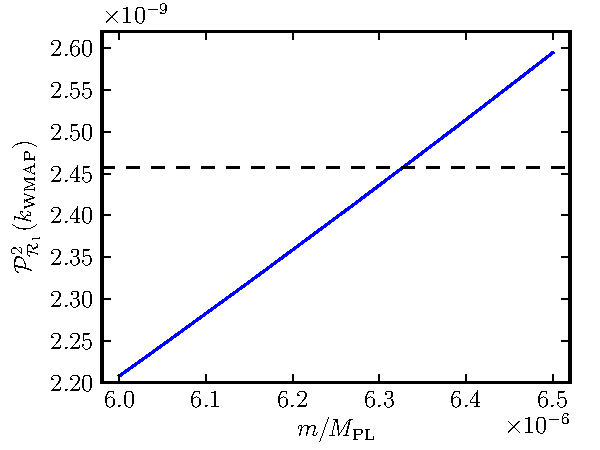
\includegraphics[width=0.43\textwidth]{numerical/graphs/msqphisq_params-small}
}\qquad%
\subfloat[Fixing $\lambda$ for $V(\vp)=\lambdaphifour$]{
 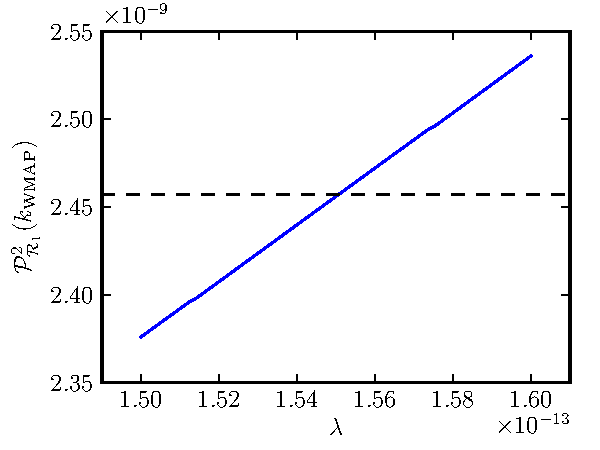
\includegraphics[width=0.43\textwidth]{numerical/graphs/lambdaphi4_params-small}
}\\%
\subfloat[Fixing $\lambda$ for $V(\vp)=\hybridtwoandfour$]{
 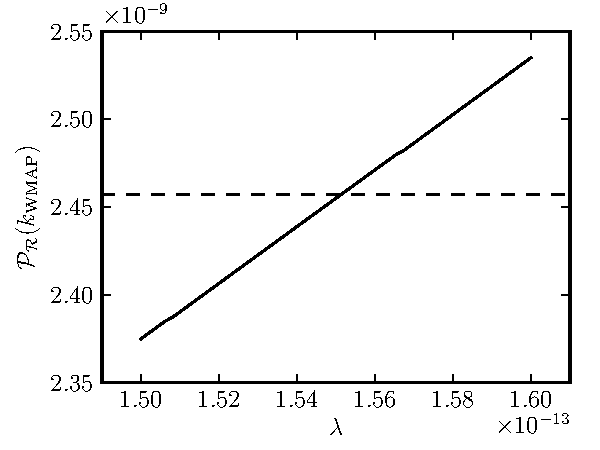
\includegraphics[width=0.43\textwidth]{numerical/graphs/hybrid2and4_params-small}
}\qquad%
\subfloat[Fixing $\lambda$ for $V(\vp)=\linde$]{
 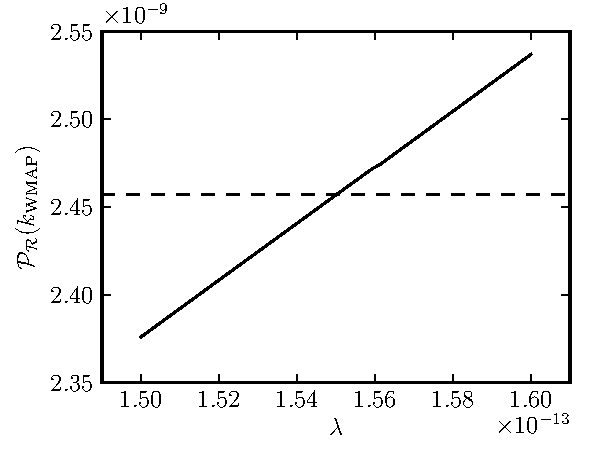
\includegraphics[width=0.43\textwidth]{numerical/graphs/linde_params-small}
}\\%
\subfloat[Fixing $\lambda$ for $V(\vp)=\phitwooverthree$]{
 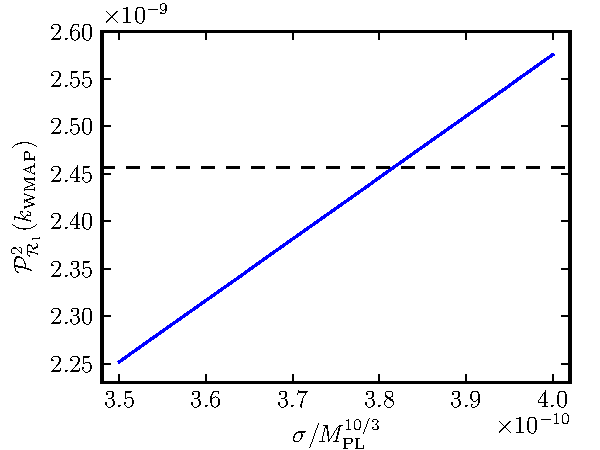
\includegraphics[width=0.43\textwidth]{numerical/graphs/phi2over3_params-small}
}
\caption[Parameter values for different potentials]{Parameter values for the
different potentials are chosen fixing $\Pr$ using WMAP5 data.}
\label{fig:params-num}
\end{figure}


% % % % % % % % % % % % % % % % % % % % % % % % % % % % % % % % 
% =========================================================== %
% % % % % % % % % % % % % % % % % % % % % % % % % % % % % % % %
\section{Initial Conditions} 
\label{sec:initconds-num}
% % % % % % % % % % % % % % % % % % % % % % % % % % % % % % % % 
% =========================================================== %
% % % % % % % % % % % % % % % % % % % % % % % % % % % % % % % %

The background system requires initial conditions for $\vp_{0},
\dN{\vp_{0}}$ and $H$. These initial conditions and the range of
e-foldings to be simulated must be selected with the choice of
potential in mind. Not only must the
e-folding range include an inflationary period, but the $k$ modes to
be calculated at first and second order must begin inside the horizon
during this range. For example the initial conditions $\vp_0 = 18\Mpl,
\dN{\vp_0} = -1 \Mpl, H = 4.65\e{-5}\Mpl$ for the $\msqphisq$ model 
give the background evolution described below and shown in Figure~\ref{fig:eps}.


The initial conditions are set for each $k$ mode a few e-foldings
before horizon crossing. This follows the example of Salopek
\etal
\cite{Salopek:1988qh} and is justified on the basis that the mode is
sufficiently inside the
horizon for the Minkowski limit to be taken. This initial time,
$n_{\mathrm{init}}(k)$, is calculated to be when
%  
\begin{equation}
 \frac{k}{aH|_{\mathrm{init}}} = 50 \,.
\end{equation}
%
The range of e-foldings being used must include the starting point for
all $k$ modes, but the parameter on the right hand side, here chosen to
be 50, can be changed if needed.  We use the small wavelength solution
of the first order equations as the initial conditions \cite{Salopek:1988qh}, with
%
\begin{eqnarray}
\label{eq:foics}
 \dvp1|_{\mathrm{init}} &=& \frac{\sqrt{8\pi G}}{a}
\frac{e^{-i k\eta}}{\sqrt{2k}} \,,\\
 \dN{\dvp1}|_{\mathrm{init}} &=& -\frac{\sqrt{8\pi G}}{a}
\frac{e^{-i k\eta}}{\sqrt{2k}} \left(1 + i \frac{k}{a H}\right) \,,
\end{eqnarray}
%
where the conformal time $\eta$ can be calculated from $\eta=\int \d\N/aH \simeq
-(aH(1-\epsilon_H))^{-1}$, when $\epsilon_H$ changes slowly. For example $\kwmap$ is initialised
about $65$ e-foldings before the end of inflation and crosses the horizon about $5$ e-foldings
later.
We also use these formulae in the calculation of the source term in \eq{eq:KG2-source-ntime} to
determine the value of $\dvp1$ for a $k$ mode before its evolution starts.


We are interested in the production of second order effects by the
evolution of the the gaussian first order modes and we make no
assumptions about the existence of second order perturbations before
the simulation begins. Therefore we set the initial condition for each second order
perturbation mode to be $\dvp2=0, \dN{\dvp2}=0$ at
the time when the corresponding first order perturbation is initialised.



% % % % % % % % % % % % % % % % % % % % % % % % % % % % % % % % 
% =========================================================== %
% % % % % % % % % % % % % % % % % % % % % % % % % % % % % % % %
\section{Implementation} 
\label{sec:impl-num}
% % % % % % % % % % % % % % % % % % % % % % % % % % % % % % % % 
% =========================================================== %
% % % % % % % % % % % % % % % % % % % % % % % % % % % % % % % %


The current implementation of the code is mainly in Python and uses the
Numerical and Scientific Python modules for their strong compiled array support
\cite{scipy}. The core of the model computation is a customised
Runge-Kutta 4th order method (see for example Eq.~(25.5.10) in
\cite{abramowitz+stegun}).  Following
Refs.~\cite{Martin:2006rs,Ringeval:2007am} the numerical calculation
proceeds in four stages. The background equation (\ref{eq:bgntime}),
rewritten as two first order (in the time derivative) equations, is
evolved from the specified initial state until some end time required
to be after the end of the inflationary regime.  The end of inflation
occurs when $\d^2a/\d t^2$ is no longer positive and the parameter
$\varepsilon_H = -\dN{H}/H$ first becomes greater than or equal to $1$
(see Figure~\ref{fig:eps}). Here, this specifies a new end time for the 1st
order run, although the simulation can run beyond the strict end of
inflation if required. The initial conditions for the first order
system are then set as outlined above.
%
\begin{figure}
\centering
 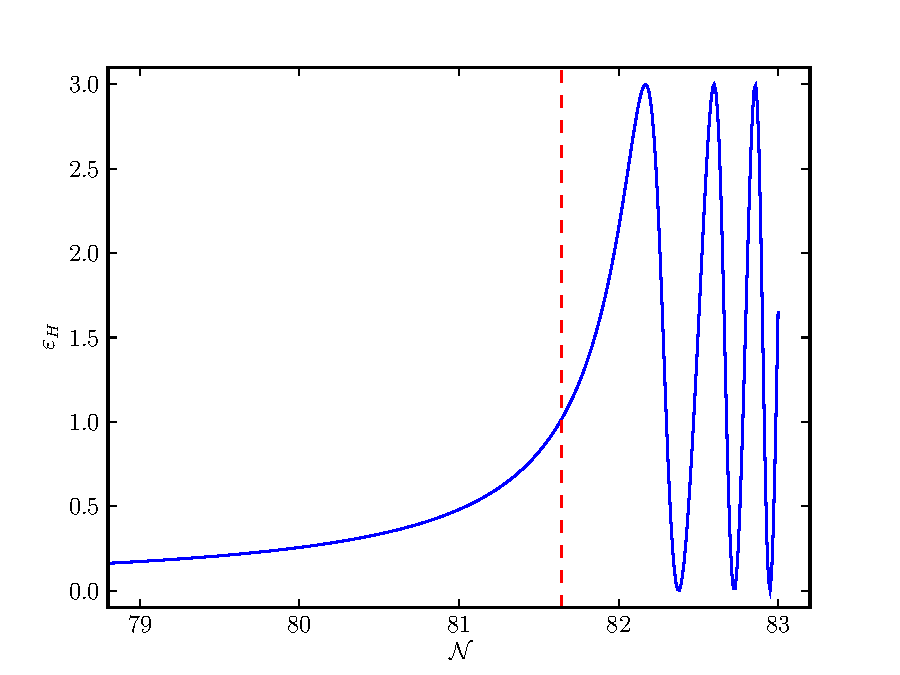
\includegraphics[width=\textwidth]{./numerical/graphs/bgepsilon}
 \caption[Plot of $\varepsilon_H$ near the end of inflation]{The end of inflation is
determined by calculating when
   $\varepsilon_H=-\dN{H}/H=1$ (red dashed line). Along the $x$-axis,
   $\N$ is the number of e-foldings from the start of the
   simulation.}
\label{fig:eps}
\end{figure}

The system of ordinary differential equations for the first order
perturbations from \eq{eq:fontime} is calculated using a standard
Runge-Kutta method. A fixed time step method is used in order to
simplify the construction of the  second order source term and because
\emph{a priori} it is not known which time steps would be required at
second order if an adaptive time step system were used. The first
order equations are separable in terms of $k$ and so it is
straightforward to run multiple instances of the system and collate
the results at the end. However, as will be discussed below, the first
order calculation is not computationally expensive in comparison with
the other stages and takes of the order of a few minutes for around
$8000$ time steps and $1025$ $k$ modes.


Once the first order system has been solved 
the source term for the second order system must be calculated. As the
real space equation for the source involves terms quadratic in the
first order perturbation it is necessary to perform a convolution in
Fourier space, as shown in \eq{eq:KG2-fourier-sr-aterms}.  Transforming
back into real space was not considered due to the presence of both
gradient operators and their inverses. Here the slow roll version of
the source term integrand has been used, but the method can equally be
applied to the full equation. This stage is the most computationally
intensive and can be run in parallel as each time step is independent
of the others. The nature of the convolution integral and the
dependence of the first order perturbation on the absolute value of
its arguments requires that twice as many $k$ modes are calculated at
first order than are desired at second order as explained above.  As
the first order calculation is computationally cheaper than the source
term integration, this does not significantly lower the possible
resolution in $k$-space, which is still limited by the source term
computation time.  Once the integrand is determined it is fed into a
Romberg integration scheme. As for $\theta$  which was
discretised by $N_\theta$ points in \eq{eq:AtoD-num}, this requires that the
number of $k$ modes is
%
\begin{equation}
\label{eq:nk-constraint-num}
N_k=2^l + 1\,,
\end{equation}
%
for some\footnotemark $l\in\mathbb{N}$. 
\footnotetext{The number of discretised $k$ modes $N_k$ does not need to be equal to
  $N_\theta$.}
This requirement can be lifted by opting for a less
accurate and somewhat slower standard quadrature routine.


The second order system is finally run with the source term and other
necessary data being read as required from the memory or disk. The
Runge-Kutta method calculates half time steps for each required point,
for example if $y(x_n)$ is known and $y(x_{n+1})=y(x_n+h)$ is required
(for step size $h$), the method will calculate the derivatives of $y$
at $y(x_n), y(x_n +h/2)$ and $y(x_n + h)$. As we need to specify the
source term at every calculated timestep, the requested timestep for
the second order method must be twice that used at first order.  This decreases the
accuracy of the method but does not require the use
of splines and interpolation techniques to determine background and
1st order variables between time steps.


The second order system is similar in run time to the first order 
system but the
source integration is more complex, involving the
integration of $N_k^2\times N_\theta$ values at
each time step.
Although a large amount of data is produced at each step at this
stage for 
each of the wavenumbers $k$, only the integrated result is stored to be used
in the second order run.
Results for each stage are stored in the open HDF5 standard which can deal
efficiently with large
files and is very portable, allowing data analysis independent of the
Python/Numpy programming environment.
We intend to release the program under a suitable license once the code has
matured and some of the improvements discussed in Section \ref{sec:disc-num} have
been implemented.


% % % % % % % % % % % % % % % % % % % % % % % % % % % % % % % % 
% =========================================================== %
% % % % % % % % % % % % % % % % % % % % % % % % % % % % % % % %
\section{Code Tests}
\label{sec:tests-num}
% % % % % % % % % % % % % % % % % % % % % % % % % % % % % % % % 
% =========================================================== %
% % % % % % % % % % % % % % % % % % % % % % % % % % % % % % % %


We have tested the numerical code in a variety of controlled
circumstances in order to quantify the effect of different choices of
parameters. In particular it is important to know whether the values
picked for $N_\theta$, the number of discretised $\theta$s, $\Delta k$, the size of the
spacing of the discretised $k$ modes, and the range of
$k$ values significantly impacts on the results. The ODE solving parts
of the code are straightforward and follow standard algorithms.


As mentioned above the WMAP results \cite{Komatsu:2008hk} use
observations in the range $k\in [0.92 \e{-60}, 3.1 \times
  10^{-58}]\Mpl = [3.5\e{-4}, 0.12] M_{\mathrm{pc}}^{-1}$. We will
consider three different $k$ ranges both in our results and the tests
of the code\footnotemark:
%
\begin{eqnarray}
\label{eq:Krangedefns}
K_1 &=& \left[1.9\e{-5}, 0.039\right]\Mpc^{-1}\,,\quad \Delta k = 3.8\e{-5}\Mpc^{-1}
\,,\nonumber\\
K_2 &=& \left[5.71\e{-5}, 0.12\right]\Mpc^{-1}\,, \quad \Delta k = 1.2\e{-4}\Mpc^{-1}\,,
\nonumber\\ 
K_3 &=& \left[0.52\e{-5}, 0.39\right]\Mpc^{-1}\,, \quad \Delta k = 3.8\e{-4}\Mpc^{-1} \,.
\end{eqnarray}
% 
\footnotetext{The $k$ ranges in $\Mpl$ are:
\begin{eqnarray*}
\label{eq:Krangedefns-mpl}
K_1 &=& \left[0.5\e{-61}, 1.0245\e{-58}\right]\Mpl\,,\quad \Delta k = 1\e{-61}\Mpl \nonumber\\
K_2 &=& \left[1.5\times 10^{-61}, 3.0735\e{-58}\right]\Mpl\,, \quad \Delta k = 3\e{-61}\Mpl
\nonumber\\ 
K_3 &=& \left[0.25\e{-60}, 1.02425\e{-57}\right]\Mpl\,, \quad \Delta k = 1\e{-60}\Mpl \,.
\end{eqnarray*}
}
% 
The first, $K_1$, has a very fine resolution but covers only a small portion of the WMAP range. 
The next, $K_2$, is closest to the WMAP range with a still quite fine resolution.  The final
range, $K_3$, has a larger $k$ mode step size $\Delta k = 1\e{-60}\Mpl = 3.8\e{-4}\Mpc^{-1}$ and
covers a greater range than the others, extending to much smaller scales than WMAP can observe.

\begin{figure}
\centering
% 
 \subfloat[Relative error for different $N_\theta$][The relative error for different
$N_\theta$, the number of
discretised $\theta$s, keeping the other parameters fixed and using the $K_3$
range. The upper blue line ($N_\theta=129$) and middle green line
 ($N_\theta=257$) have relative errors at least an order of magnitude larger
than the lower red line ($N_\theta=513$).]{
 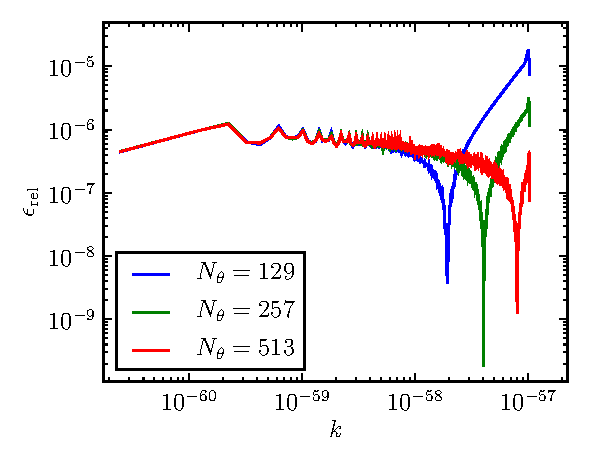
\includegraphics[width=0.43\textwidth]{numerical/graphs/err-nthetas-small.pdf}
 \label{fig:err-nthetas}
}\qquad
% 
\subfloat[Relative error for three different $k$ ranges][The relative error for the 3
different $k$ ranges $K1$, $K2$,
$K3$ (starting from the left). The parameter $\Delta k$
is set equal to $1\e{-61}\Mpl, 3\e{-61}\Mpl, 1\e{-60}\Mpl$ respectively.]{
 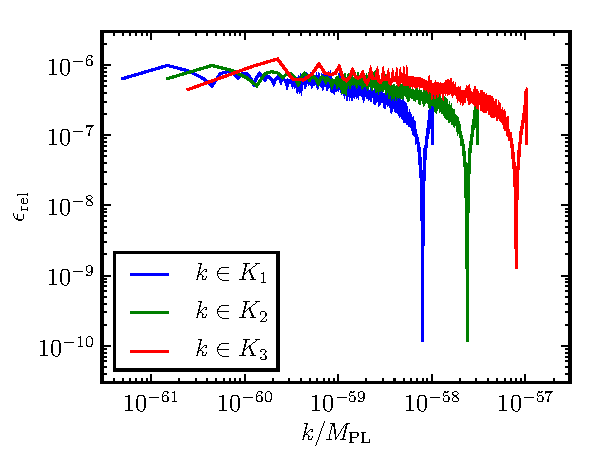
\includegraphics[width=0.43\textwidth]{numerical/graphs/err-kranges-small.pdf}
 \label{fig:err-kranges}
}
% 
\caption[Two figures comparing relative errors]{Comparison of relative errors for
different $N_\theta$ and $k$ ranges.}
\label{fig:err-comparison}
\end{figure}

The main new addition in the code is the calculation of the
convolution of the perturbations for the source term
\eq{eq:KG2-source-ntime}. In particular the first of the $\theta$ dependent terms in
\eq{eq:AtoD-num}, $A$,
can be convolved analytically for certain smooth $\dvp1(k)$s. 
 We take $\dvp1(k)$ to be similar in form to the initial conditions
(\ref{eq:foics}), for example $\dvp1(k)\propto 1/\sqrt{k}$ with proportionality constant
$\alpha$.
If $I_A$ denotes the convolution of the $A$ term:
% 
\begin{equation}
 I_A (k) = 2\pi \int_{\kmin}^{\kmax} q^2 \dvp1(q) A(k, q) \d q \,,
\end{equation}
% 
then putting in $\dvp1(k) = \alpha/\sqrt{k}$ gives
% 
\begin{equation}
 I_A(k) = 2\pi \alpha^2 \int_{\kmin}^{\kmax} \d q\, q^{\frac{3}{2}}
\int_{0}^{\pi} \d\theta\, (k^2 + q^2 -2k q \cos{\theta})^{-4} \sin{\theta}\,. 
\end{equation}
% 
This has the analytic solution
% 
\begin{eqnarray}
\label{eq:err-analytic-num}
 A(k) &=& \frac{\pi}{18}\frac{\alpha^2}{k} \left\{ 
3k^3\left[\log\left(2\sqrt{k}\right) - \frac{\pi}{2}  + 
\arctan\left(\sqrt{\frac{\kmin}{k-\kmin}}\right) 
 + \log\left(2\left(\sqrt{\kmin} + \sqrt{\kmin + k}\right)\right) \right.\right. \nonumber \\
&& \left. -\, \log\left(2\left(\sqrt{\kmax} + \sqrt{\kmax + k}\right)\right) 
  - \log\left(2\left(\sqrt{\kmax} + \sqrt{\kmax - k}\right)\right) \right]  \nonumber \\
&& +\, \sqrt{\kmax}\left[\sqrt{\kmax -k} \left(-3k^2 + 14k\kmax - 8\kmax^2\right)  
 + \sqrt{\kmax +k} \left(3k^2 + 14k\kmax + 8\kmax^2\right)\right] \nonumber \\ 
&& \left. -\, \sqrt{\kmin}\left[\sqrt{k -\kmin} \left(3k^2 - 14k\kmax + 8\kmax^2\right) 
 - \sqrt{k +\kmin} \left(3k^2 + 14k\kmax + 8\kmax^2\right)\right] \right\} \,.
\end{eqnarray}
%
We have tested our code against this analytic solution for various
combinations of $k$ ranges and $N_\theta$. The relative error
%
\begin{equation}
 \epsilon_\mathrm{rel} = \frac{|\mathrm{analytic}- \mathrm{calculated} |}{|\mathrm{analytic}|}
\end{equation}
%
is small for all the tested cases but certain combinations of
parameters turned out to be better than others. The relative error of
all the following results is not affected by the choice of $\alpha$ so
we will keep it constant throughout.

\begin{figure}
 \centering
 \includegraphics[width=\textwidth]{numerical/graphs/err-deltak4.pdf}
 \caption[Relative error in the convolution term $A$]{The relative error in
convolution term $A$ for different values of $\Delta k$.
The other parameters are fixed: $\kmin=1\times10^{-60}\Mpl, N_k = 1025$ and $N_\theta=513$. The
upper 
blue line ($\Delta k=1\e{-61}\Mpl$ and middle green line ($\Delta k=3\e{-61}\Mpl$) have relative
errors at
least an order of magnitude larger than the lower red line ($\Delta k=1\e{-60}\Mpl$).}
 \label{fig:err-deltaks}
\end{figure}


We first tested the effect of changing $N_\theta$, the number of
samples of the $\theta$ range $[0,\pi]$.  Figure~\ref{fig:err-nthetas}
plots these results for the $k$ range $K_3$ with $\Delta k =
1\e{-60}\Mpl$. Only three values of $N_\theta$ are shown for clarity. It
can be seen that increasing $N_\theta$ decreases the relative error (for the convolution
term at least) when the other parameters are kept constant, as one
might expect.


As mentioned above the choice of $k$ range is especially important as
the convolution of the terms depends heavily on the minimum and
maximum values of this range. Indeed this is clear from the analytic
solution in \eq{eq:err-analytic-num}. Figure~\ref{fig:err-kranges}
shows the difference in relative error for the three different $k$
ranges described above with 
% Mpc values 
$\Delta k= 3.8\e{-5}, 1.2\e{-4}$ and $3.8\e{-4}\Mpc^{-1}$
% Mpl values
($\Delta k= 1\e{-61}, 3\e{-61},1\e{-60}\Mpl$)
respectively. The accuracy is similar in all three cases.


Another important check is whether the resolution of the $k$ range is
fine enough. Varying $\Delta k$ can not be done in isolation of
course, if the constraint for $N_k$, \eq{eq:nk-constraint-num},
is to
be met. For this test the end of the $k$ range changed with $\Delta k$
but the other parameters were kept fixed as $\kmin=1\e{-60}\Mpl=3.8\e{-4}\Mpc^{-1},
N_k = 1025$ and $N_\theta=513$. Figure~\ref{fig:err-deltaks} plots
these results again for only three indicative values.  For $\Delta
k<\kmin$, here the upper two lines, there is a marked degradation in
the accuracy of the method. This is understandable as many
interpolations of multiples of $\Delta k$ below $\kmin$ will be set to
$0$. Once $\Delta k$ is greater than $\kmin$ the relative error is
very similar for higher values (not shown in the figure).


\begin{figure}
 \centering
 \includegraphics[width=\textwidth]{numerical/graphs/err-deltak-kmin.pdf}
 % err-deltak-kmin.pdf: 432x324 pixel, 72dpi, 15.24x11.43 cm, bb=
 \caption[Relative error of the convolution term with fixed $\kmin$]{The 
relative error of the convolution term for three different values of $\Delta k$. In
contrast to Figure~\ref{fig:err-deltaks} $\kmin=1\e{-61}\Mpl=3.8\e{-5}\Mpc^{-1} \le \Delta k$ for
each.}
 \label{fig:err-deltak-kmin}
\end{figure}


It should be noted that these tests show the relative errors in the
computation of the $A$ convolution term, the most straightforward term in \eq{eq:AtoD-num}, only and
do not
represent
errors for the full calculation. However, they show that at least for
the pure convolution term the accuracy is good compared with the
analytic results. Equation (\ref{eq:err-analytic-num}) gives some indication of
the difficulty involved in finding an analytic solution for the other
terms, although this is a goal for future work. Having described the
implementation and accuracy of the numerical system we will outline
our results in the next section.
 
% 
% 
% 

% % % % % % % % % % % % % % % % % % % % % % % % % % % % % % % % 
% =========================================================== %
% % % % % % % % % % % % % % % % % % % % % % % % % % % % % % % %
\section{Discussion}
\label{sec:disc-numerical}
% % % % % % % % % % % % % % % % % % % % % % % % % % % % % % % % 
% =========================================================== %
% % % % % % % % % % % % % % % % % % % % % % % % % % % % % % % %
